\section{Introduction}
\begin{frame}{Balloon Model}
\begin{figure}
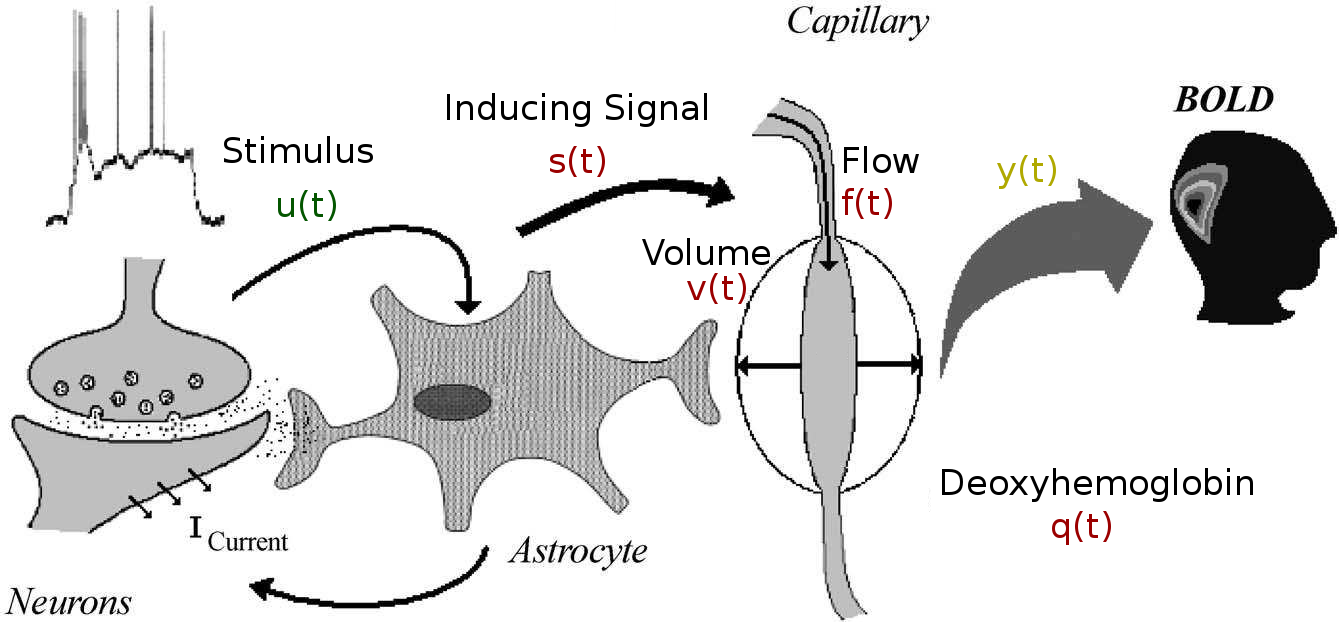
\includegraphics[width=10cm]{model2}
\caption{
    \tiny
    \cite{Riera2003}
}
\end{figure}
\note{Its been known for about 20 years that changes in Blood Oxygen Level alter
        T2$^*$ relaxation times. The basis of contrast in fMRI is 
        changes in the so-called spin-spin relaxation (or T2$^*$ relaxation time
        of tissue). The rate of loss in nuclear spin coherence depends on the molecules in the voxel being
        measured \emph{and the surrounding voxels}. For this reason the signal 
        detected from BLOOD doesn't just depend on the amount of oxygen, but also the
        amount of De-oxygenated hemoglobin. The question then, is what drives changes
        in De-oxygenated Hemoglobin and blood volume?
        
        Well the brain has no local oxygen storage, so it is completely dependent on 
        fresh Oxygenated-Hemoglobin. When the brain becomes more active, firing rates
        for neurons increase by several orders of magnitude, and recharging these neurons
        requires additional oxygen for matabolism. }
\note{Rates from below 1 Hz to 5 to 6 Hundred Hz}
\note{Change in average firing rates increase metabolism and sympathetic response causes
        increased inflow of oxygenated blood.}
\note{In the version of the Balloon model I used, the flow is locked to metabolism.}
\note{According the balloon model this increases the local blood volume, and the outflow pressure.}
\note{So the signal is altered by changes in the ratio of Deoxyhemoglobin and Oxygenated Hemoglobin,
        which are a function of Volume and Oxygenation.}
\end{frame}

\begin{frame}{Activation Chain}
\begin{figure}
    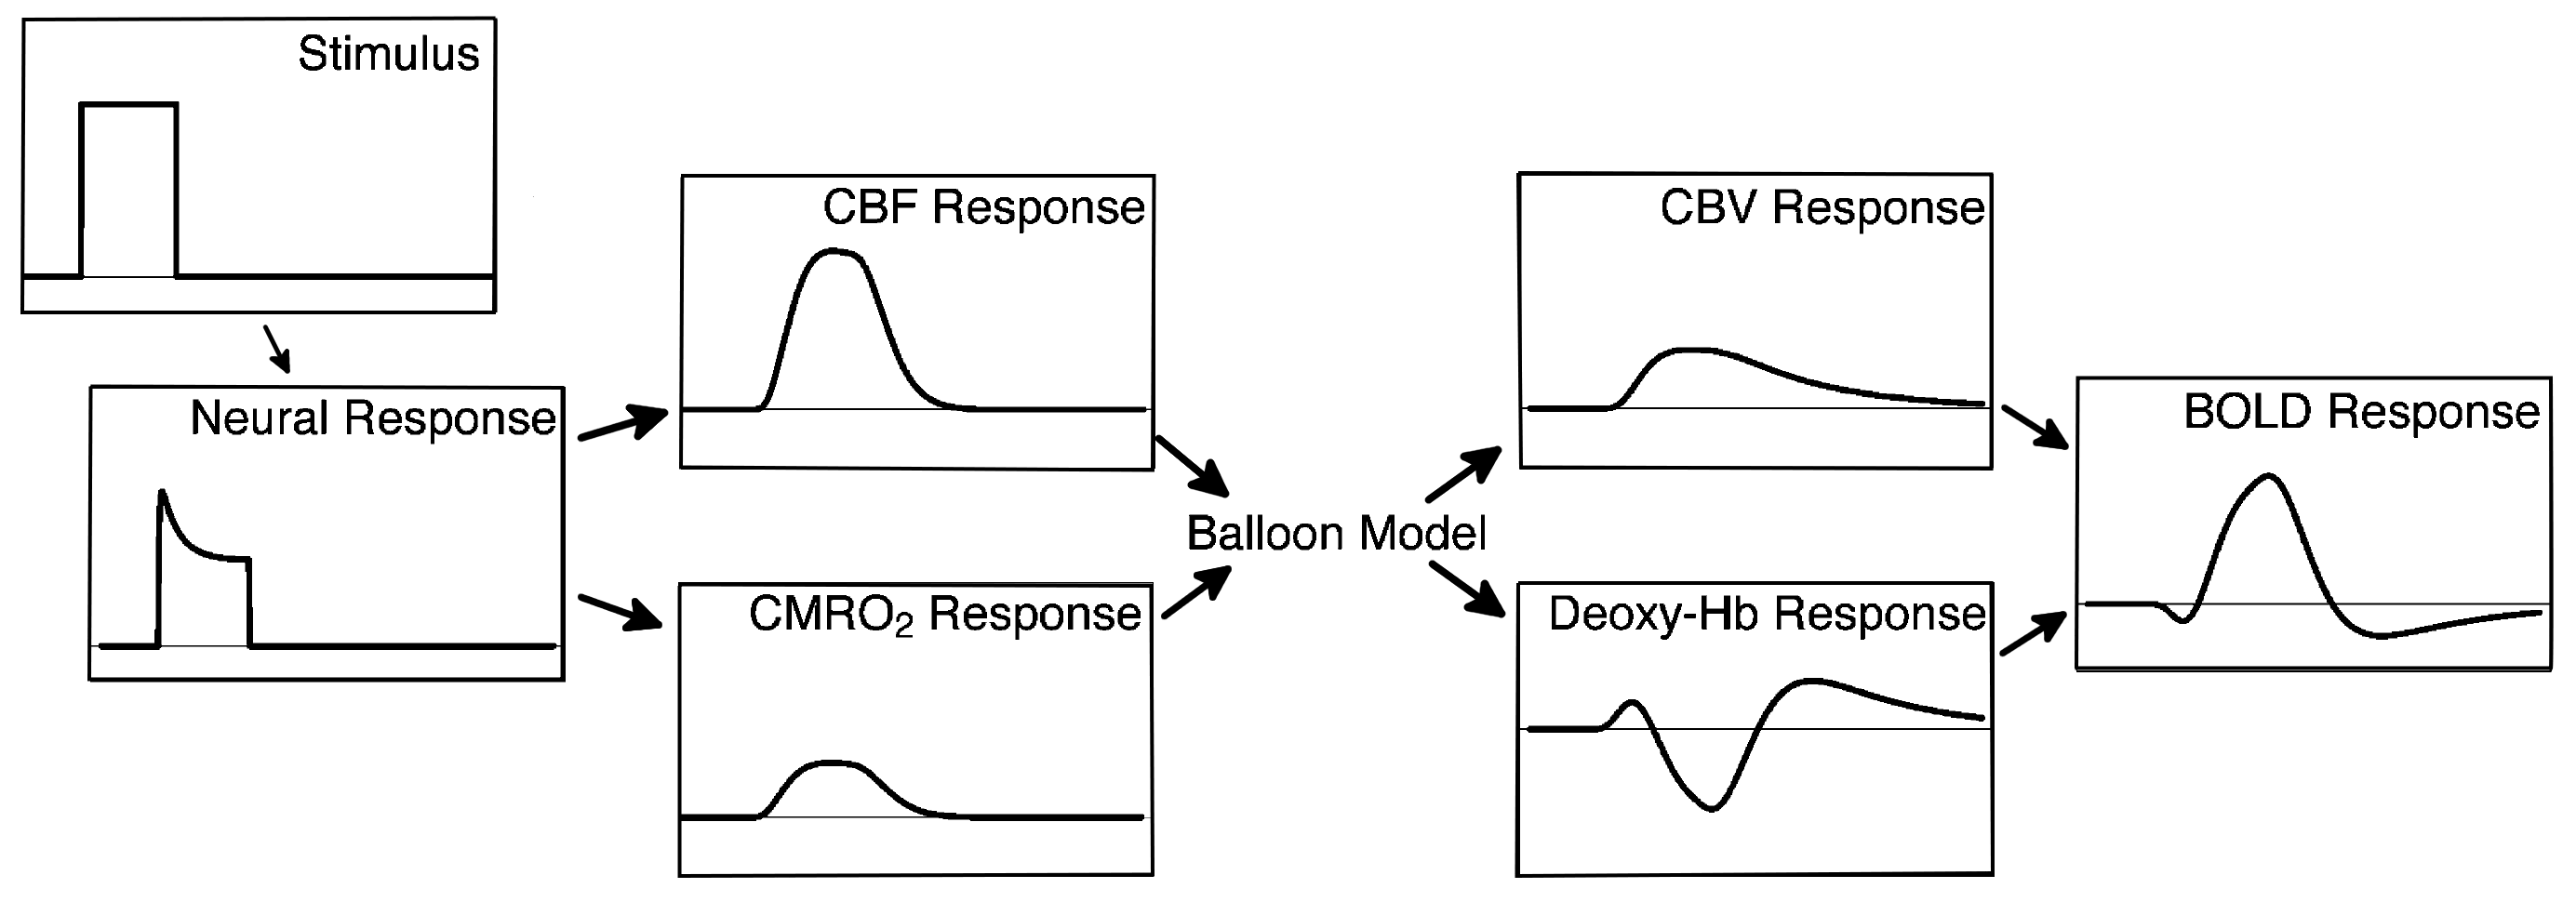
\includegraphics[width=\textwidth]{graphs}
\caption{
    \tiny
    \cite{Buxton2004}
}
\end{figure}
\end{frame}

%more expansion of all the parameters
\begin{frame}{BOLD State Space Model}
  \scriptsize
  \begin{columns}
  \begin{column}{.7\textwidth}
    \begin{itemize}
    \item State Vector:
    \begin{eqnarray}
    \color{mblue}\dot{s}(t) &=& {\color{mred}\epsilon} {\color{mgreen}u(t)} - 
                \frac{\color{mblue}s(t)}{\color{mred}\tau_s} - \frac{{\color{mblue}f(t)}-1}{\color{mred}\tau_f} \nonumber \\
    \color{mblue}\dot{f}(t) &=& \color{mblue}s \nonumber \\
    \color{mblue}\dot{v}(t) &=& \frac{{\color{mblue}f(t)} - 
                {\color{mblue}v(t)} ^ {1/{\color{mred}\alpha}}}{\color{mred}\tau_0} \nonumber \\
    \color{mblue}\dot{q}(t) &=& \frac{1}{\color{mred}\tau_0}
            \left(\frac{{\color{mblue}f(t)}(1-(1-{\color{mred}E_0})^{1/\color{mblue}f(t)})}{\color{mred}E_0} -
        \frac{\color{mblue}q(t)}{{\color{mblue}v(t)}^{1-1/\color{mred}\alpha}}\right) \nonumber 
    \end{eqnarray}
    \item Output:
    $${\color{myellow}y(t)} = {\color{mred}V_0}(a_1( 1 - {\color{mblue}Q(t)}) - a_2(1 - {\color{mblue}V(t)}))$$
    \end{itemize}
  \end{column}

  \begin{column}{.3\textwidth}
    \begin{itemize}
        \item State Variables:
        $${\color{mblue}s(t)}, {\color{mblue}f(t)}, {\color{mblue}v(t)}, {\color{mblue}q(t)}$$
        \item Parameters:
        $${\color{mred}\epsilon}, {\color{mred}\tau_s}, {\color{mred}\tau_f}, {\color{mred}\alpha}, 
                    {\color{mred}\tau_0}, {\color{mred}E_0}, {\color{mred}V_0}$$
        \item Constants:
        $$a_1, a_2$$
        \item Input:
        $$\color{mgreen}u(t)$$
    \end{itemize}
  \end{column}
  \end{columns}
  \note{System is dissipative:\\
  If no input is provided, it will rather quickly decay.\\
  Constant input leads to steady state response.\\
  First term in $\dot{q}$ is the metabolism term.\\
  Outflow is the $v^{1/\alpha}$ term\\
  Significant nonlinearity.}
\end{frame}
